%!TEX root = ./report.tex
\newpage
\appendix
\section{Results of Black Box Tests}
\label{app:blackboxtests}
%Test
%VERY IMPORTANT TODO: mention which test buildings were used and where they can be found.
\subsection{Cases:}
For these tests, we have several cases: One of them is a subset of a real IFC model, provided by Kaj J\o rgensen. The rest have been created by Mathias Demant for our testing, and do not represent any real buildings. The files can be found in Prototype/Model2ModelWorkflows/NanoLabBuilding/ on the attached medium. The results can be seen in Figures \ref{fig:test1}, \ref{fig:test2}, \ref{fig:test3}, and \ref{fig:test4}.
\subsection{Tests:}
For each case, we will perform the following tests between the two MWE2 workflows:
\subsubsection{Test 1:}
Modifying the metadata (name, description) for one of each of the three product types (wall, opening, flow segment).
\textbf{Expected result:} The output IFC model differs from the input IFC model in that it has altered metadata (name, description).
\subsubsection{Test 2:}
Modifying the placement of one of each of the three products types.
\textbf{Expected result:} A new IFCLocalPlacement object now exists in the IFC output model with the modified metadata. 
\subsubsection{Test 3:}
Modifying the list of walls in a opening element
\textbf{Expected result:} A new IFCRelVoidElement is present in the output IFC model, compared to the input mode, linking the wall and opening.
\subsubsection{Test 4:}
Deleting one Pipe.
\textbf{Expected result:} The output IFC model no longer contains the deleted flow segment. Any created orphans should be garbage collected.
\subsubsection{Test 5:}
Adding one opening.
\textbf{Expected result:} The output IFC model should now contain the created opening, along with any new objects referenced by the opening (LocalPlacement, Axis2Placement3d)
\subsubsection{Test 6:}
Adding one opening, deleting one flow segment, and modifying metadata for one wall.
\textbf{Expected result:} The output IFC model should now contain the created opening (along with referenced objects), the flow segment should be deleted (along with orphans), and the metadata for the wall should be updated.
\begin{figure}[ht]
    \centering
        \centerline{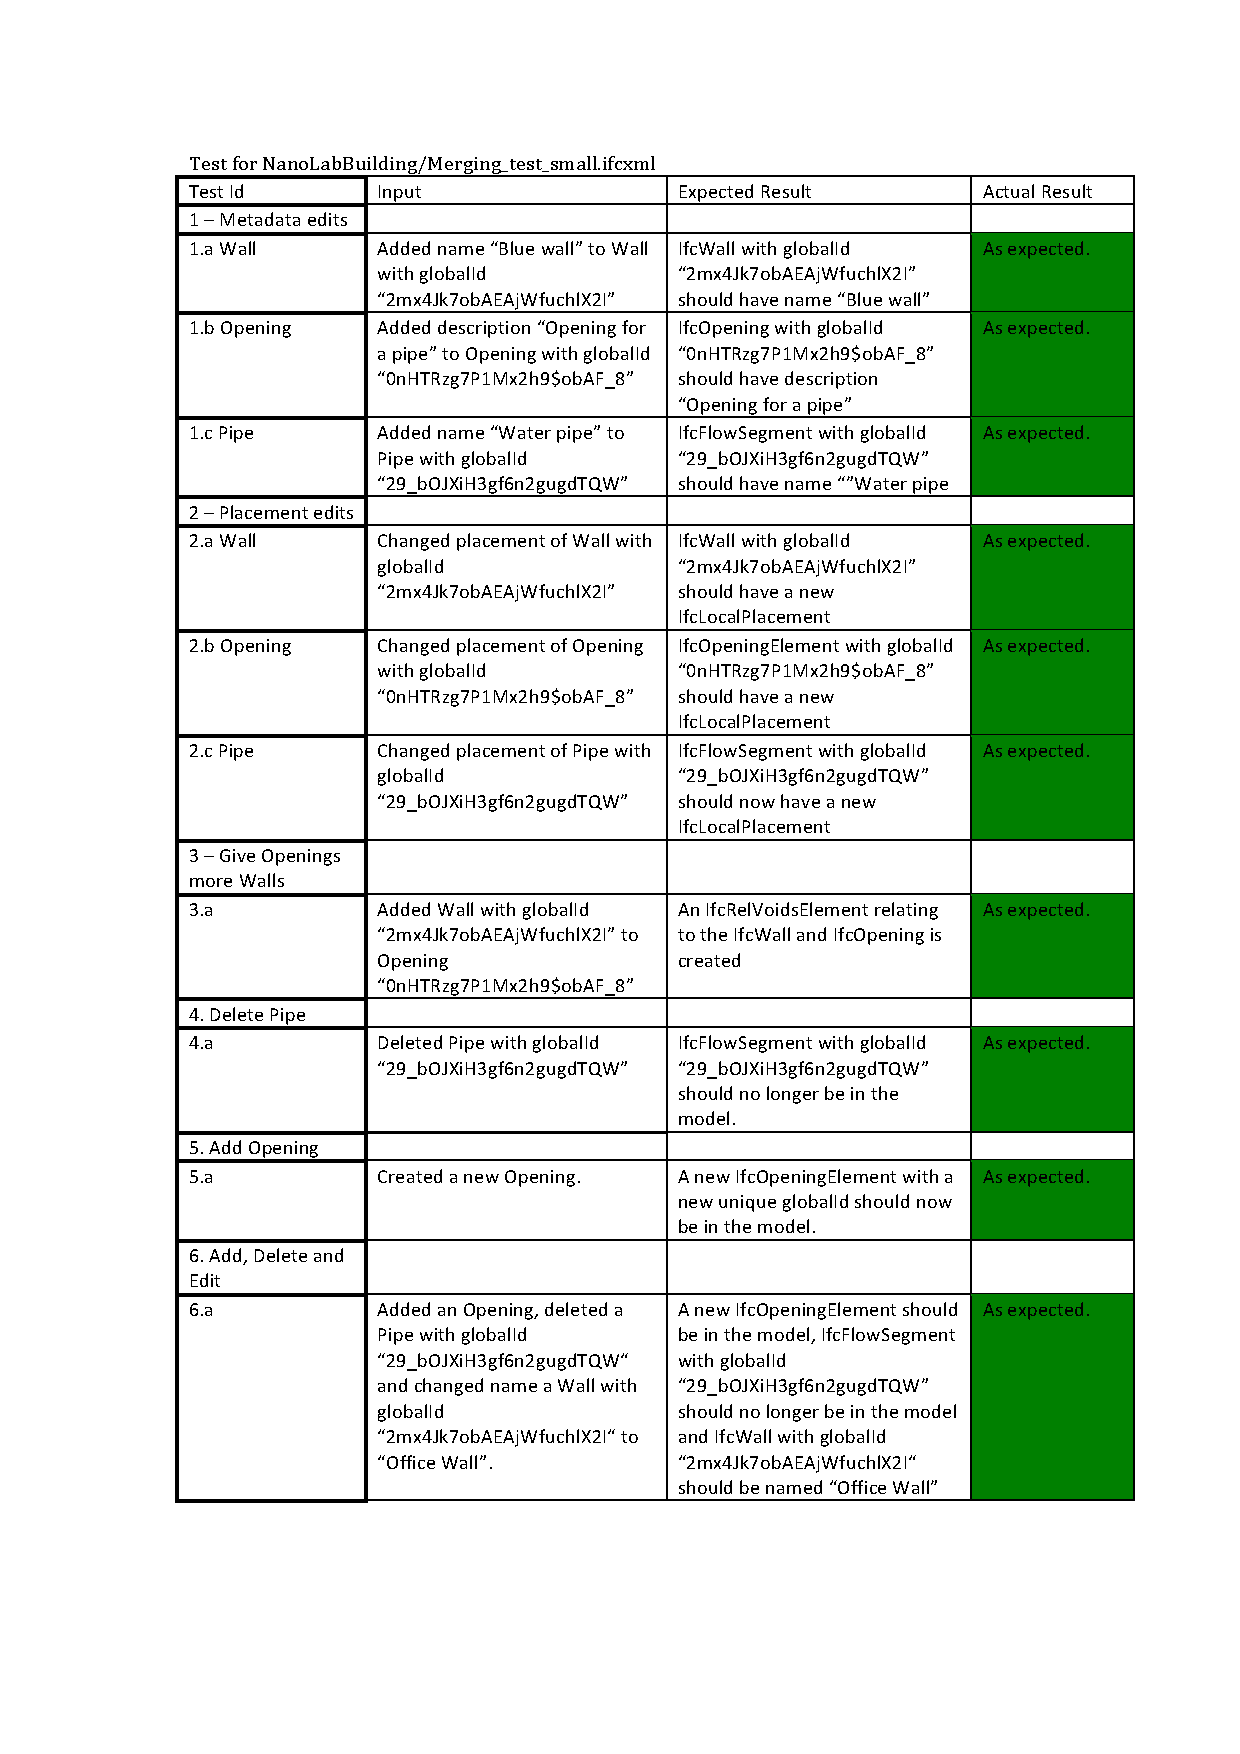
\includegraphics[width=150mm]{images/Test1.pdf}}
    \caption{}
    \label{fig:test1}
\end{figure}
\begin{figure}[ht]
    \centering
        \centerline{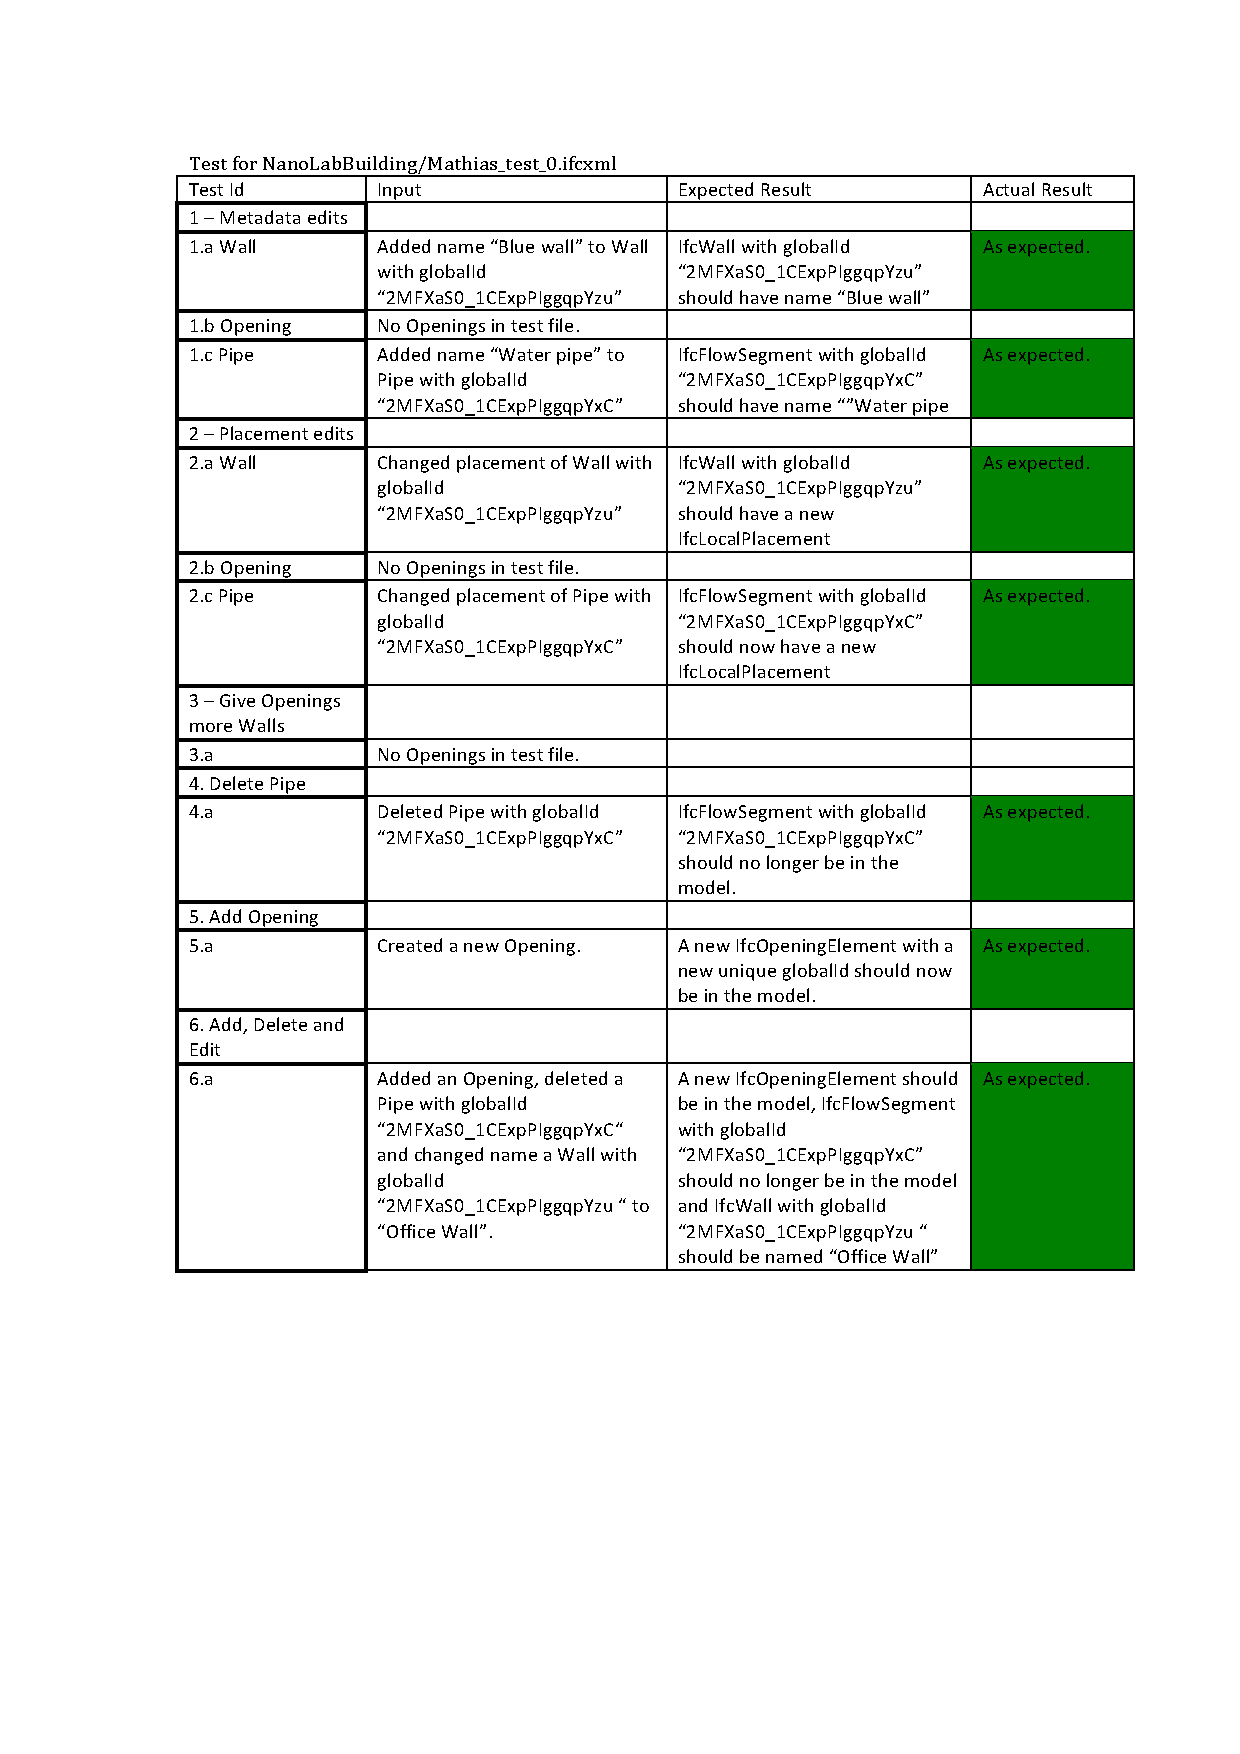
\includegraphics[width=150mm]{images/Test2.pdf}}
    \caption{}
    \label{fig:test2}
\end{figure}
\begin{figure}[ht]
    \centering
        \centerline{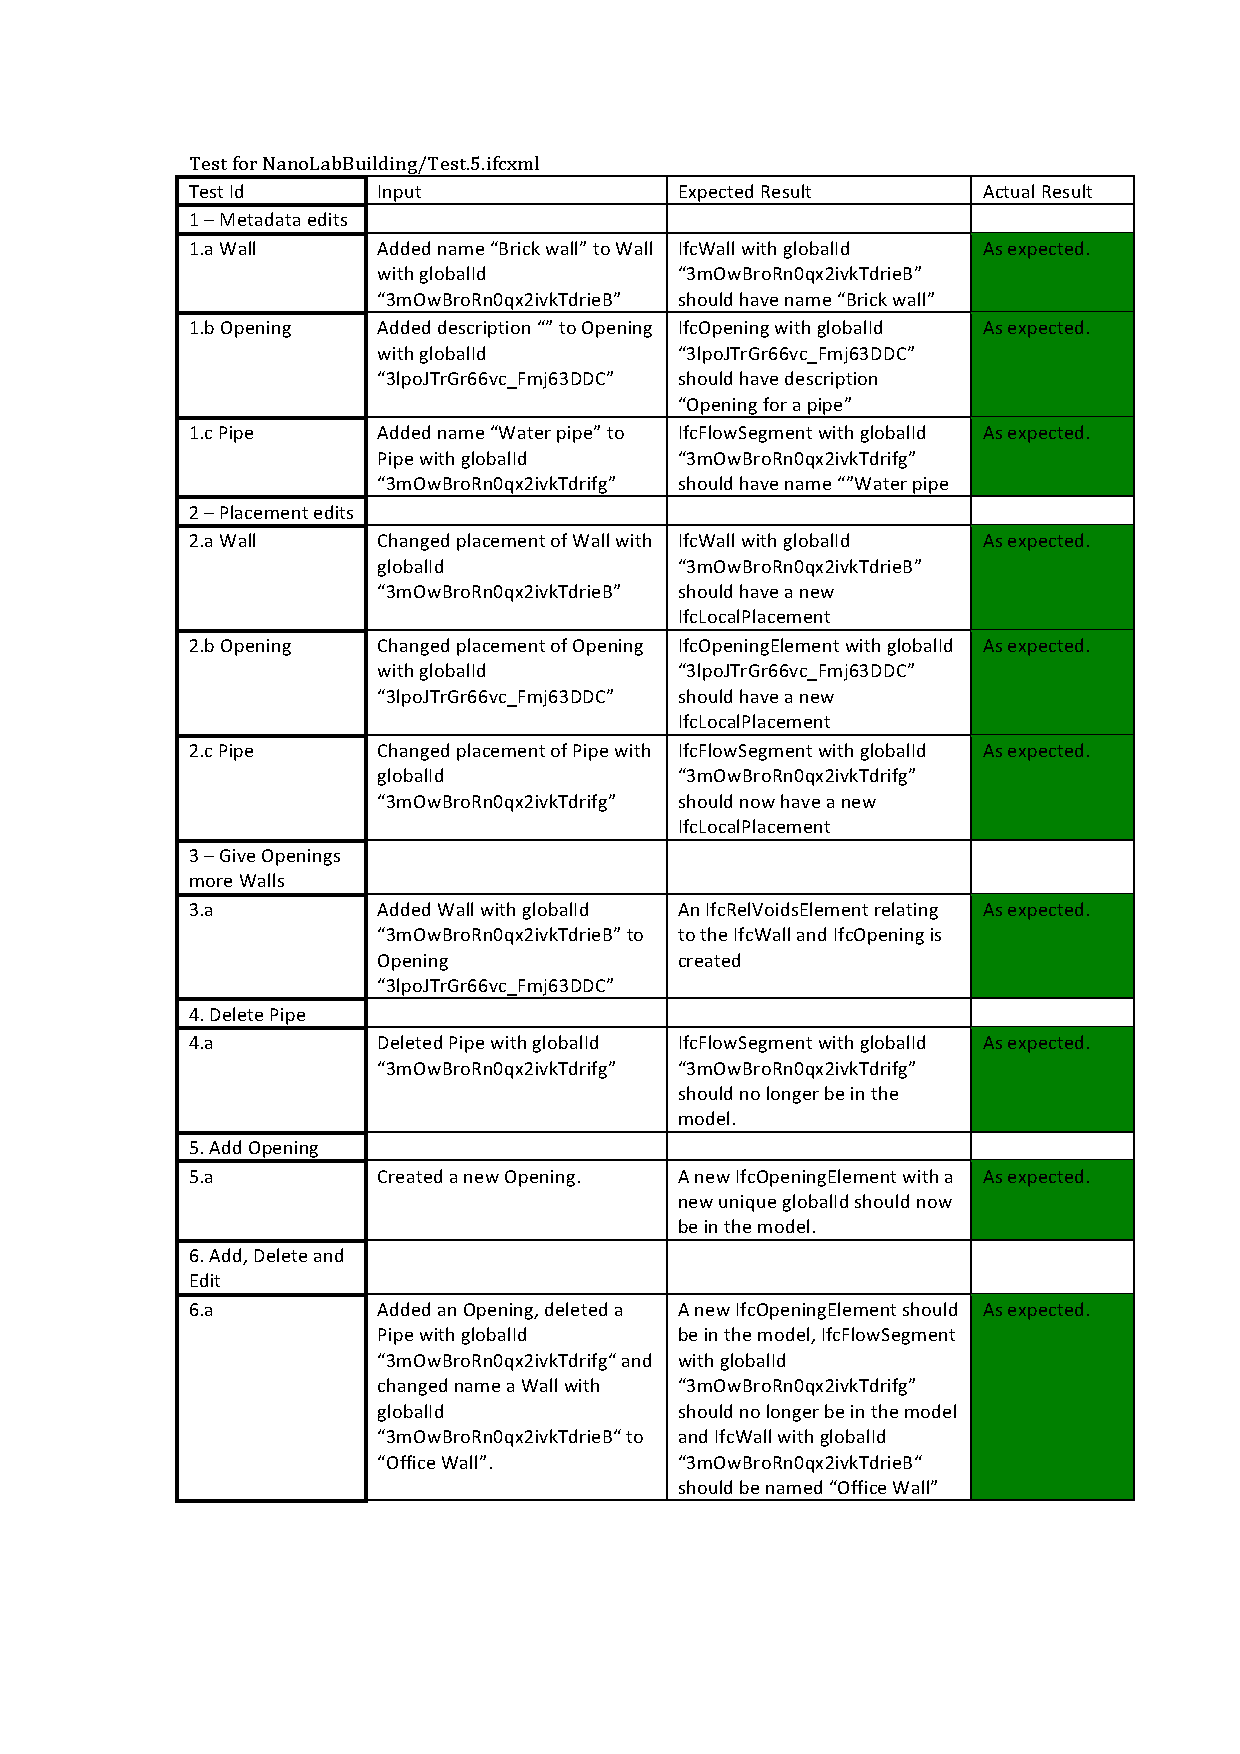
\includegraphics[width=150mm]{images/Test3.pdf}}
    \caption{}
    \label{fig:test3}
\end{figure}
\begin{figure}[ht]
    \centering
        \centerline{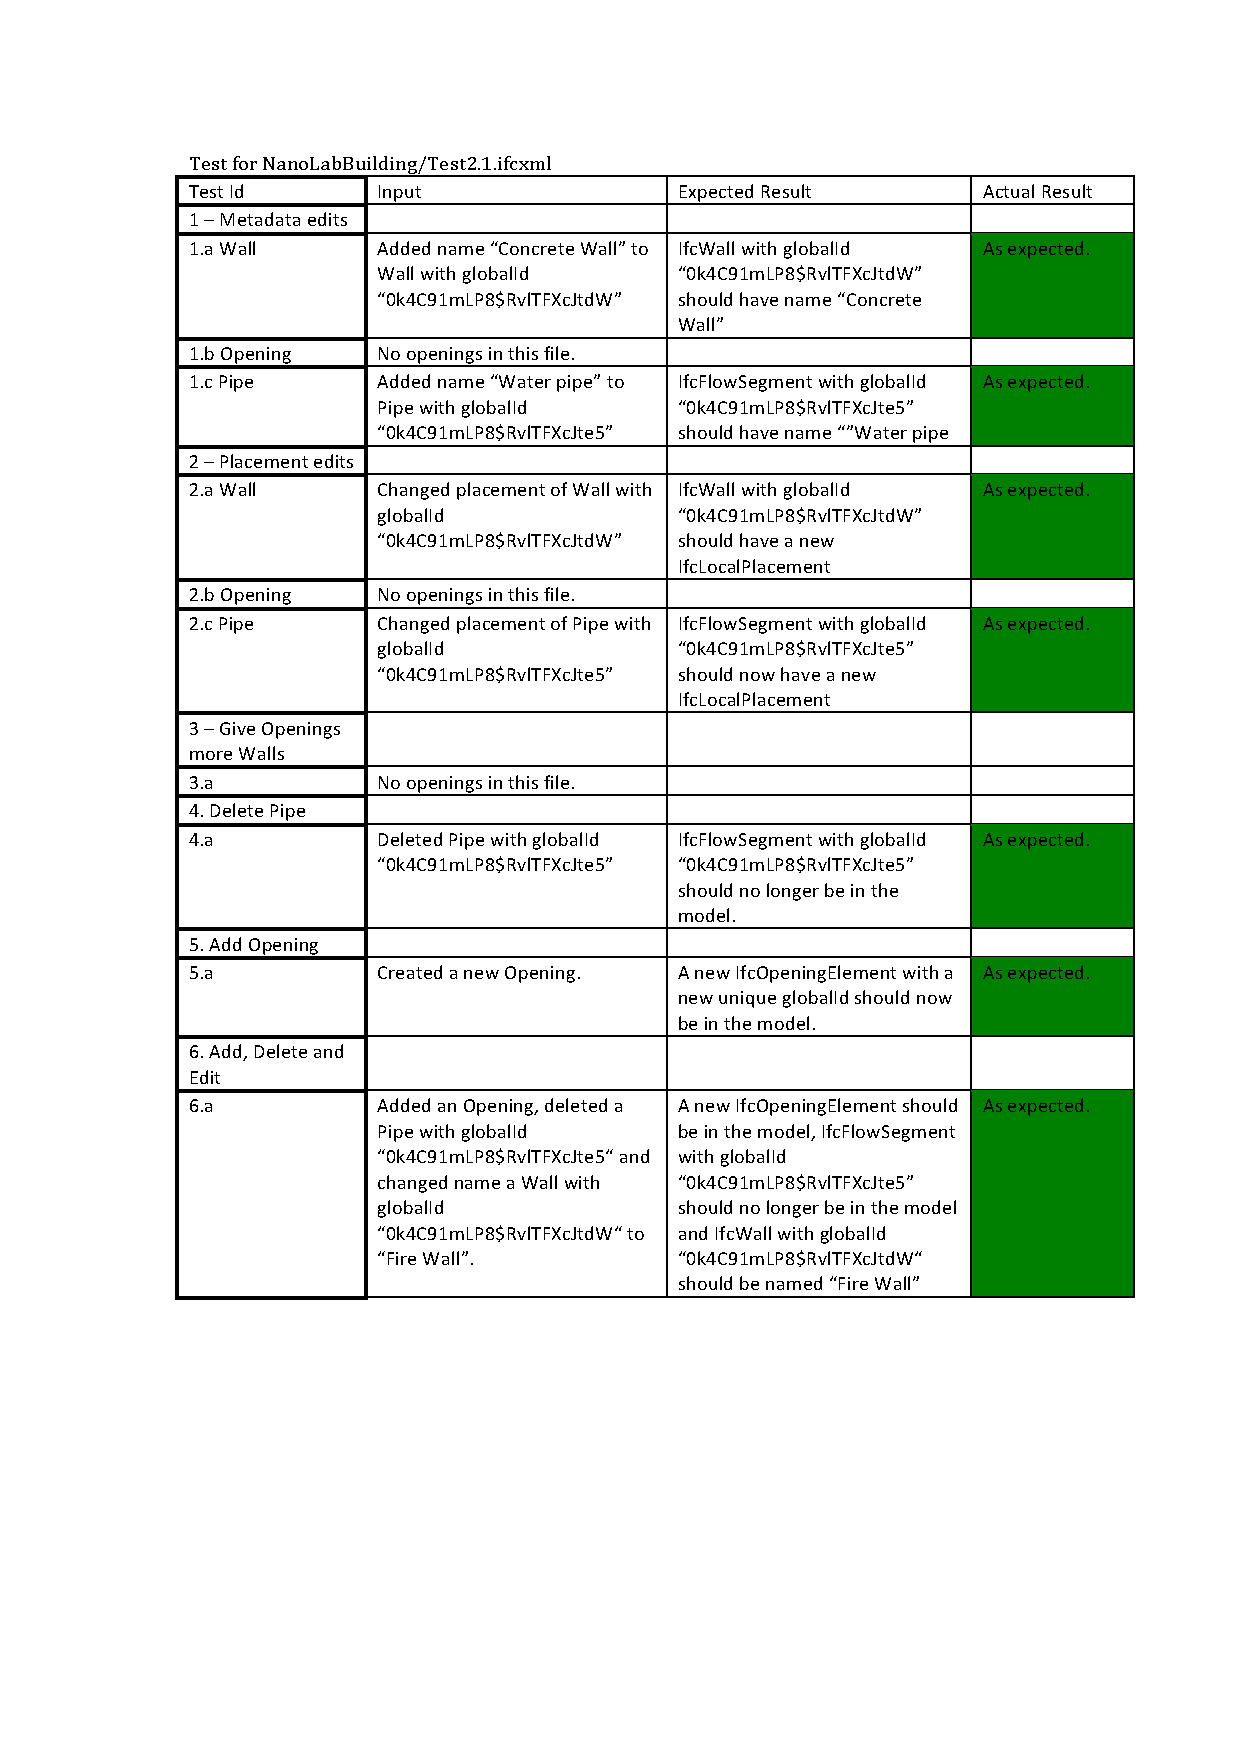
\includegraphics[width=150mm]{images/Test4.pdf}}
    \caption{}
    \label{fig:test4}
\end{figure}


\section{Automated Tests}
\label{app:automatedtests}
The workflow components used for tests can be found in the Eclipse project under: Model2ModelWorkflows/src/tests. These components work as a part of two test workflows similar to the ones used in the actual prototype. The only difference is that test components have been inserted after extraction and transformation components. The IFC2Pipes.mwe2 workflow is thus tested by the IFC2PipesTest.mwe2 workflow and the Pipes2IFC.mwe2 workflow is tested by the Pipes2IFCTest.mwe2 workflow.

\subsubsection{Testing Element Extraction}
The TestIFCExtractor workflow component verifies that the extraction process executed with a correct result. On any input building it checks that the number of extracted IfcProducts correspons to the number of products that should be extracted by looking directly at the ifcXML. For each of the extracted product elements it tests for a valid GUID and ID. On all input models of Appendix \ref{app:blackboxtests} the test passes.

\subsubsection{Testing IFC to Pipes Model Transformation}
The following consistency verification between elements in the IFC and Pipes models are carried out:

\begin{itemize}
	\item IfcFlowSegment <-> FlowSegment
	\item IfcOpening <-> Opening
	\item IfcWall <-> Wall
	\item IfcLocalPlacement <-> LocalPlacement
	\item IfcAxis2Placement3d <-> Axis2Placement3D
	\item IfcDirection <-> Direction
\end{itemize}

By going through all extracted IFC products after the model to model transformation and comparing them to the elements of the Pipes model, the TestTransformers test component automates transformation testing of the subdomain. All consistency tests on all input buildings from Appendix \ref{app:blackboxtests} pass the tests.

\subsubsection{Testing Pipes to IFC Update Routine}
The TestTransformer test component is used for the purpose of testing the Pipes to IFC Update Routine as well. The same consistency checks are performed after the Pipes2IFCTransformer, which performs this routine. The same element relations, as above, are tested. All consistency tests on all input buildings from Appendix \ref{app:blackboxtests} pass the tests.





